\subsection{球}\label{subsec:2-5}

\subsubsection{球的概念和性质}

\begin{wrapfigure}[8]{r}{4.5cm}
    \centering
    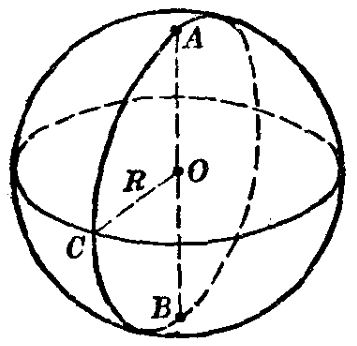
\includegraphics[width=4cm]{../pic/ltjh-ch2-42.png}
    \caption{}\label{fig:ltjh-2-42}
\end{wrapfigure}

常见的排球、足球及滚珠等物体,都呈球形。

半圆以它的直径为旋转轴,旋转所成的曲面叫做\zhongdian{球面}。
球面所围成的几何体叫做\zhongdian{球体},简称\zhongdian{球}。
半圆的圆心叫做\zhongdian{球心}。
连结球心和球面上任意一点的线段叫做\zhongdian{球的半径}。
连结球面上两点并且经过球心的线段叫做\zhongdian{球的直径}。
如图 \ref{fig:ltjh-2-42} 的球中,点 $O$ 是球心,线段 $OC$ 是球的半径,线段 $AB$ 是球的直径。

球面也可以看作与定点(球心)的距离等于定长(半径)的所有点的集合(轨迹)。

一个球用表示它的球心的字母来表示,例如球 $O$。

用一个平面去截一个球,截面是圆面。 球的截面有下面的性质:

\zhongdian{(1)球心和截面圆心的连线垂直于截面(图 \ref{fig:ltjh-2-43} 甲);}

\zhongdian{(2)球心到截面的距离 $\bm{d}$ 与球的半径 $\bm{R}$ 及截面的半径 $\bm{r}$,有下面的关系:
    \jiange $$ \bm{r = \sqrt{R^2 - d^2}} \juhao $$
}

当 $d = 0$ 时,截面经过球心, $r = R$。
这时,球面被截得的圆最大(图 \ref{fig:ltjh-2-43} 乙),这个圆叫\zhongdian{球的大圆}。
不经过球心的截面所截得的圆叫做\zhongdian{球的小圆}。

\begin{figure}[htbp]
    \centering
    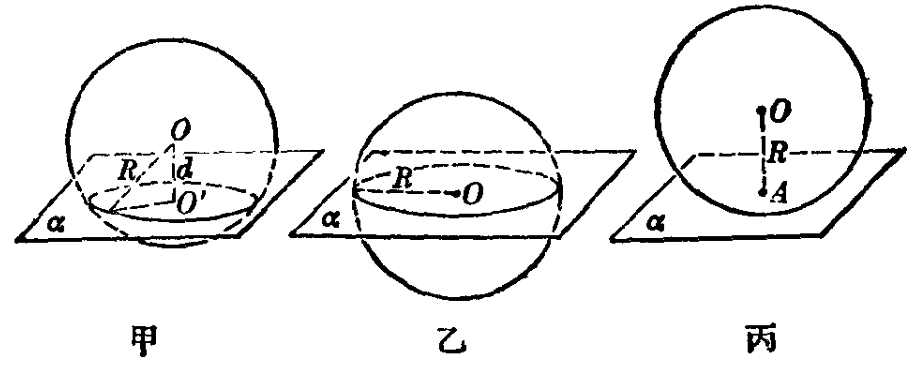
\includegraphics[width=11cm]{../pic/ltjh-ch2-43.png}
    \caption{}\label{fig:ltjh-2-43}
\end{figure}

当 $d = R$ 时,$r = 0$,截面缩成一点。 这个点是截平面与球的唯一公共点。
和球只有一个公共点的平面叫做\zhongdian{球的切面}(图 \ref{fig:ltjh-2-43},丙)。
球与它的切面的公共点叫做\zhongdian{切点}。

当我们把地球看作一个球时,经线就是球面上从北极到南极的半个大圆。
赤道是一个大圆,其余的纬线都是小圆(图 \ref{fig:ltjh-2-44})。

\begin{figure}[htbp]
    \centering
    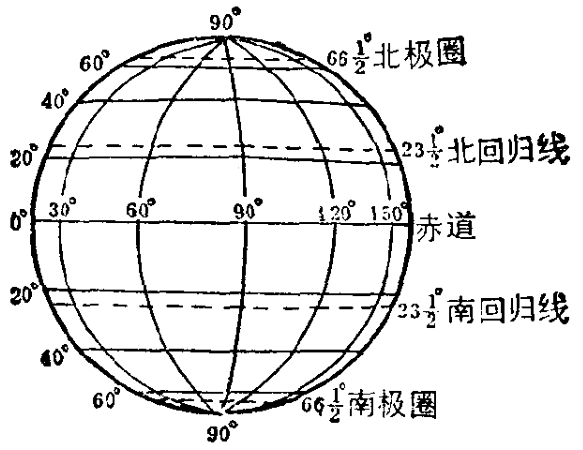
\includegraphics[width=7cm]{../pic/ltjh-ch2-44.png}
    \caption{}\label{fig:ltjh-2-44}
\end{figure}

在球面上,两点之间的最短距离,就是经过这两点的大圆在这两点间的一段劣弧的长度。
我们把这个弧长叫做\zhongdian{两点间的球面距离}。
例如,图 \ref{fig:ltjh-2-45} 中的 $PQ$ 的长度就是 $P$、$Q$ 两点间的球面距离。
飞机、轮船都是尽可能以大圆弧为航线航行。

\begin{figure}[htbp]
    \centering
    \begin{minipage}[b]{7cm}
        \centering
        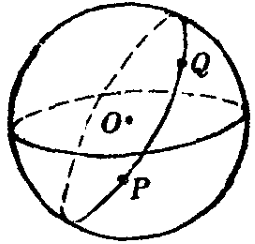
\includegraphics[width=4cm]{../pic/ltjh-ch2-45.png}
        \caption{}\label{fig:ltjh-2-45}
    \end{minipage}
    \qquad
    \begin{minipage}[b]{7cm}
        \centering
        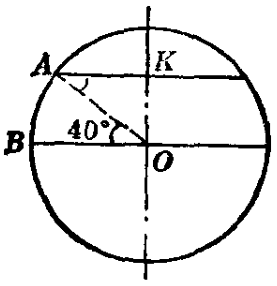
\includegraphics[width=4cm]{../pic/ltjh-ch2-46.png}
        \caption{}\label{fig:ltjh-2-46}
    \end{minipage}
\end{figure}

\liti 我国首都北京靠近北纬 $40^\circ$。求北纬 $40^\circ$ 纬线的长度约为多少 km(地球半径约 6370 km)。

\jie 如图 \ref{fig:ltjh-2-46}, $A$ 是北纬 $40^\circ$ 圈上的一点,$AK$ 是它的半径,所以 $OK \perp AK$。
设 $c$ 是北纬 $40^\circ$ 的纬线长,因为 $\angle AOB = \angle OAK = 40^\circ$,所以

\hspace*{4em} $\begin{aligned}
    c &= 2\pi \cdot AK \\
      &= 2\pi \cdot OA \cos OAK \\
      &= 2\pi \cdot OA \cos 40^\circ \\
      &\approx 2 \times 3.142 \times 6370 \times 0.7660 \\
      &\approx 3.066 \times 10^4 (\qianmi) \juhao
\end{aligned}$

答:北纬 $40^\circ$ 纬线的长度约为 $3.066 \times 10^4$ km。


\subsubsection{球的直观图的画法}

\begin{wrapfigure}[8]{r}{5.5cm}
    \centering
    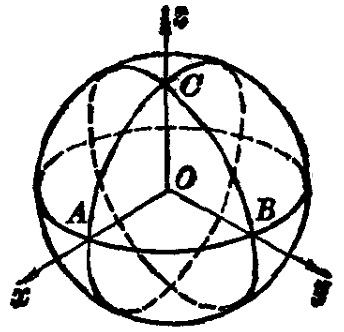
\includegraphics[width=5cm]{../pic/ltjh-ch2-47.png}
    \caption{}\label{fig:ltjh-2-47}
\end{wrapfigure}

球的直观图,一般采用正等测画法。 这时球的轮廓是一个圆。

\liti 画半径为 $R$ 的球的直观图。

\huafa (1) 画轴 \quad 经过点 $O$ 画 $x$ 轴、$y$ 轴、$z$ 轴,轴间角为 $120^\circ$(图 \ref{fig:ltjh-2-47})。

(2)画大圆 \quad 以 $O$ 为中心,分别按 $x$ 轴、$y$ 轴,$y$ 轴、$z$ 轴,$z$ 轴、$x$ 轴
画半径为 $R$ 的圆的直观图(三个椭圆)。

(3)成图 \quad 以点 $O$ 为圆心画一个圆与三个椭圆都相切。
最后经过整理,就得到球的直观图。


\subsubsection{球的表面积}

圆柱、圆锥、圆台的表面积公式,都是利用它们的展开图求出的。
由于球面不能展开成平面图形,所以球的表面积公式无法用展开图求出。
为了求得球的表面积公式,我们来证明一个预备定理:

\begin{dingli}[定理][dl:qmnjyt-cmj]
    球面内接圆台(圆台上、下底面是球的两个平行截面)的高为 $\bm{h}$,球心到母线的距离为 $\bm{p}$,
    那么圆台的侧面积为 $\bm{2\pi ph}$。
\end{dingli}

已知:球面 $O$ 的内接圆台的高 $O_1O' = h$,球心 $O$ 到母线 $AD$ 的距离 $OE = p$(图 \ref{fig:ltjh-2-48} 甲)。

\begin{figure}[htbp]
    \centering
    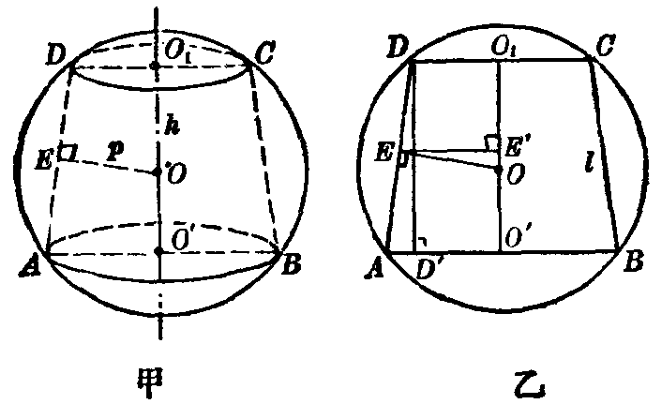
\includegraphics[width=10cm]{../pic/ltjh-ch2-48.png}
    \caption{}\label{fig:ltjh-2-48}
\end{figure}

求证: $S_\text{圆台侧} = 2\pi ph$。

\begin{enhancedline}

\zhengming 过圆台的轴的平面 截圆台和球分别得轴截面 $ABCD$ 和球的大圆 $\yuan\,O$。
这时 $ABCD$ 是 $\yuan\,O$ 的内接等腰梯形(图 \ref{fig:ltjh-2-48} 乙)。

作 $OE \perp AD$,垂足 $E$ 是 $AD$ 的中点,$OE = p$。
再作 $DD' \perp AB$、$EE' \perp O_1O'$,垂足分别是 $D'$、$E'$,那么 $DD' = h$。

设圆台上、下底面半径为 $r'$、$r$,母线长为 $l$,则
$$ EE' = \exdfrac{1}{2} (r' + r) \juhao $$

由于两个直角三角形 $ADD'$ 和 $OEE'$ 的对应角相等,(为什么?)
所以 $\triangle ADD' \xiangsi \triangle OEE'$。

$\therefore$ \quad $l:h = p:\exdfrac{1}{2}(r + r')$, \qquad $l(r + r') = 2ph$。\\
代入圆台侧面积公式,得到
\zhongdian{$$ \bm{S_\text{圆台侧} = \pi (r+r')\, l = 2\pi ph} \juhao $$}

\zhuyi 这个结果对于球的内接圆柱、圆锥同样成立。
\end{enhancedline}

现在,我们来求半径为 $R$ 的球的表面积。

\begin{figure}[htbp]
    \centering
    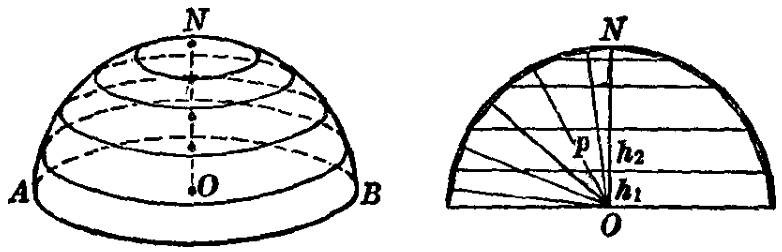
\includegraphics[width=10cm]{../pic/ltjh-ch2-49.png}
    \caption{}\label{fig:ltjh-2-49}
\end{figure}

如图 \ref{fig:ltjh-2-49},将半球面上的半大圆 $ANB$ 分成 $2n$ 等分,
用过各分点平行于半球大圆面的平面将半球分为 $n$ 部分,
以截得的圆为底作圆台、圆锥,设它们的高分别是 $h_1$、$h_2$、…、$h_n$。
球心到它们的母线的距离都为 $p$。
根据上面的预备定理,这些圆台、圆锥的侧面积的和为
\begin{align*}
    S &= 2\pi ph_1 + 2\pi ph_2 + \cdots + 2\pi ph_n \\
      &= 2\pi p (h_1 + h_2 + \cdots + h_n) \\
      &= 2\pi p \cdot ON \\
      &= 2\pi pR \juhao
\end{align*}

如果分点无限增加,侧面就无限地接近于半球面,同时 $p$ 也无限地接近于 $R$。
当 $p$ 变为 $R$ 时,侧面积的和 $S$ 变为 $2\pi R^2$。
我们把这个和作为半球面的面积,由此得到下面的定理:

\begin{dingli}[定理][dl:qm-mj]
    球面面积等于它的大圆面积的 4 倍。
    \begin{center}
        \framebox[12em]{$\bm{S_\text{球面} = 4\pi R^2}$。}
    \end{center}
    \vspace*{-2.5em}即
\end{dingli}\vspace*{1em}


\begin{enhancedline}

\begin{wrapfigure}[8]{r}{4.5cm}
    \centering
    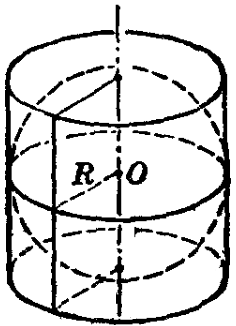
\includegraphics[width=3.5cm]{../pic/ltjh-ch2-50.png}
    \caption{}\label{fig:ltjh-2-50}
\end{wrapfigure}

\liti 已知:圆柱的底面直径与高都等于球的直径。 求证:
(1)球的表面积等于圆柱的侧面积;
(2)球的表面积等于圆柱全面积的 $\exdfrac{2}{3}$。

\zhengming (1)设球的半径为 $R$,则圆柱的底面半径为 $R$,高为 $2R$,得

\qquad $S_\text{球} = 4\pi R^2$,

\qquad $S_\text{圆柱侧} = 2\pi R \cdot 2R = 4\pi R^2$,

$\therefore$ \quad $S_\text{球} = S_\text{圆柱侧}$。

(2) $\because$ \quad $S_\text{圆柱全} = 4\pi R^2 + 2\pi R^2 = 6\pi R^2$,

\hspace{3.5em} $S_\text{球} = 4\pi R^2$,

$\therefore$ \quad $S_\text{球} = \exdfrac{2}{3} S_\text{圆柱全}$。
\end{enhancedline}

\begin{lianxi}

\xiaoti{海面上,地球球心角 $1'$ 所对的大圆弧长约为 1 海里,1 海里约是多少 km?}

\xiaoti{计算地球表面积是多少 $\pfqm$。}

\end{lianxi}



